%% ============================================================
%% THESIS SUBMISSION APPROVAL (TSA) MEETING PRESENTATION
%% Title:  Self-Adaptive Model-Based Protection for
%%         Future Power Systems
%% Author: Anoop V Eluvathingal
%% Dept:   Electrical Engineering, IIT Madras
%% Date:   June 2026
%% ============================================================

\documentclass[10pt,aspectratio=169]{beamer}

%% ── Theme & Colour ──────────────────────────────────────────
\usetheme{Madrid}
\usecolortheme{default}

%% IIT Madras dark-navy palette
\definecolor{iitmnavy}{RGB}{0,32,91}
\definecolor{iitmgold}{RGB}{179,138,0}
\definecolor{iitmred}{RGB}{180,20,20}
\definecolor{iitmblue}{RGB}{0,90,160}
\definecolor{iitmgray}{RGB}{90,90,90}

\setbeamercolor{palette primary}{bg=iitmnavy, fg=white}
\setbeamercolor{palette secondary}{bg=iitmnavy!85, fg=white}
\setbeamercolor{palette tertiary}{bg=iitmnavy!70, fg=white}
\setbeamercolor{palette quaternary}{bg=iitmnavy, fg=white}
\setbeamercolor{structure}{fg=iitmnavy}
\setbeamercolor{section in toc}{fg=iitmnavy}
\setbeamercolor{frametitle}{bg=iitmnavy, fg=white}
\setbeamercolor{title}{bg=iitmnavy, fg=white}
\setbeamercolor{block title}{bg=iitmnavy!90, fg=white}
\setbeamercolor{block body}{bg=iitmnavy!7}
\setbeamercolor{alerted text}{fg=iitmred}
\setbeamercolor{itemize item}{fg=iitmblue}
\setbeamercolor{itemize subitem}{fg=iitmblue!70}

\setbeamerfont{frametitle}{size=\normalsize, series=\bfseries}
\setbeamerfont{title}{size=\large, series=\bfseries}
\setbeamerfont{author}{size=\small}
\setbeamerfont{institute}{size=\footnotesize}
\setbeamerfont{date}{size=\footnotesize}

%% ── Packages ────────────────────────────────────────────────
\usepackage{graphicx}
\usepackage{amsmath,amssymb,bm}
\usepackage{booktabs}
\usepackage{array}
\usepackage{multirow}
\usepackage{colortbl}
\usepackage{xcolor}
\usepackage{tikz}
\usetikzlibrary{arrows.meta,positioning,shapes.geometric,fit,backgrounds}
\usepackage{pgfplots}
\pgfplotsset{compat=1.18}
\usepackage{hyperref}
\hypersetup{colorlinks=false}

%% ── Numbered item style (blue circle, no TikZ grouping) ─────
\newcommand{\bitem}[1]{%
  \makebox[16pt]{\textcolor{white}{\colorbox{iitmblue}{\bfseries\scriptsize#1}}}\,%
}

%% ── Observation box (red) ───────────────────────────────────
\newcommand{\obs}[1]{%
  {\color{iitmred}\textbf{Observation:} #1}%
}

%% ── Result box ──────────────────────────────────────────────
\newcommand{\resultitem}[2]{%
  \begin{block}{\small #1}
    \small #2
  \end{block}%
}

%% ── Convenience math macros ─────────────────────────────────
\newcommand{\kibr}{k_{\mathrm{ibr}}}
\newcommand{\Idiff}{I_{\mathrm{diff}}}
\newcommand{\Ibias}{I_{\mathrm{bias}}}
\newcommand{\PINN}{\textsc{pinn}}
\newcommand{\WAPC}{\textsc{wapc}}
\newcommand{\TMS}{\mathit{TMS}}
\newcommand{\CTI}{\mathit{CTI}}

%% ── Logo ────────────────────────────────────────────────────
\logo{
\includegraphics[height=0.65cm]{new_thesis/images/iitm-logo.png}\hspace{2pt}}

%% ── No navigation symbols ───────────────────────────────────
\setbeamertemplate{navigation symbols}{}

%% ── Footer ──────────────────────────────────────────────────
\setbeamertemplate{footline}{%
  \leavevmode%
  \hbox{%
    \begin{beamercolorbox}[wd=.40\paperwidth,ht=2.25ex,dp=1ex,left,leftskip=2ex]
      {palette primary}%
      \usebeamerfont{author in head/foot}\insertshorttitle
    \end{beamercolorbox}%
    \begin{beamercolorbox}[wd=.35\paperwidth,ht=2.25ex,dp=1ex,center]
      {palette secondary}%
      \usebeamerfont{title in head/foot}\insertshortauthor
    \end{beamercolorbox}%
    \begin{beamercolorbox}[wd=.25\paperwidth,ht=2.25ex,dp=1ex,right,rightskip=2ex]
      {palette tertiary}%
      \usebeamerfont{date in head/foot}\insertframenumber{}/\inserttotalframenumber
    \end{beamercolorbox}}%
}

%% ── Title info ──────────────────────────────────────────────
\title[SAMBP for Future Power Systems]{Self-Adaptive Model-Based Protection\\for Future Power Systems}
\author[Anoop V Eluvathingal]{Anoop V Eluvathingal\\[4pt]
  \small{\color{iitmgray}Doctoral Committee: Dr.\ K.~Shanti Swarup (Guide)}}
\institute[IIT Madras]{Department of Electrical Engineering\\
  Indian Institute of Technology Madras}
\date{Thesis Submission Approval Meeting\\June 2026}

%% ═════════════════════════════════════════════════════════════
\begin{document}

%% ─────────────────────────────────────────────────────────────
%% SLIDE 1 — Title
%% ─────────────────────────────────────────────────────────────
{
\setbeamertemplate{footline}{}
\begin{frame}[noframenumbering]
  \vspace{0.4cm}
  \begin{center}
    
\includegraphics[height=1.4cm]{new_thesis/images/iitm-logo.png}
    \vspace{0.2cm}
  \end{center}
  \titlepage
  \vspace{-0.3cm}
  \begin{center}
    \footnotesize\color{iitmgray}
    Roll No:\ EE18D203 \quad|\quad
    Thesis submitted in partial fulfilment of the requirements for the degree of
    \textit{Doctor of Philosophy}
  \end{center}
\end{frame}
}

%% ─────────────────────────────────────────────────────────────
%% SLIDE 2 — Outline
%% ─────────────────────────────────────────────────────────────
\begin{frame}{Presentation Outline}
  \begin{columns}[t]
    \column{0.48\textwidth}
      \textbf{\color{iitmnavy}Part I — Motivation \& Framework}
      \medskip
      \begin{itemize}\itemsep4pt
        \item IBR revolution \& protection crisis
        \item Research gaps \& objectives
        \item SAMBP framework overview
        \item Unified inverse-estimation core
      \end{itemize}
      \vspace{0.5cm}
      \textbf{\color{iitmnavy}Part II — Protection Modules}
      \medskip
      \begin{itemize}\itemsep4pt
        \item Adaptive line differential (87L)
        \item Generator over-current (SyncOC)
        \item Transformer differential (87T)
        \item Adaptive distance relay
        \item Microgrid mode-switching
      \end{itemize}
    \column{0.48\textwidth}
      \textbf{\color{iitmnavy}Part III — Advanced Layers}
      \medskip
      \begin{itemize}\itemsep4pt
        \item Non-blocking EKF digital twin
        \item Physics-informed fault classifier
        \item Wide-Area Protection Coordinator
        \item Cybersecurity architecture
      \end{itemize}
      \vspace{0.5cm}
      \textbf{\color{iitmnavy}Part IV — Conclusions}
      \medskip
      \begin{itemize}\itemsep4pt
        \item Summary of contributions
        \item Research outcomes
        \item Thesis content \& publications
      \end{itemize}
  \end{columns}
\end{frame}

%% ─────────────────────────────────────────────────────────────
%% SLIDE 3 — Motivation: IBR Revolution
%% ─────────────────────────────────────────────────────────────
\begin{frame}{The IBR Revolution \& the Protection Crisis}
  \begin{columns}[T]
    \column{0.54\textwidth}
      \textbf{Why conventional protection fails:}
      \medskip
      \begin{enumerate}\itemsep5pt
        \item[\bitem{1}] Grid-following inverters limit fault current to
          \textbf{1.0–1.2 pu} (vs.\ 6–8 pu for synchronous machines)
        \item[\bitem{2}] Current angle and magnitude depend on
          \textbf{control mode} and LVRT strategy — unknown to the relay
        \item[\bitem{3}] High IBR penetration (\(\kibr \to 1\)) causes
          \textbf{differential relays to mis-operate or fail to trip}
        \item[\bitem{4}] Distance zones \textbf{over-reach} due to IBR reactive
          injection; impedance locus deviates from fault trajectory
        \item[\bitem{5}] Islanded microgrids see \textbf{bidirectional}
          current reversals — directional elements are unreliable
      \end{enumerate}
    \column{0.44\textwidth}
      \begin{block}{\small IBR Penetration Trend}
        \small
        \centering
        \begin{tabular}{lcc}
          \toprule
          Scenario & $\kibr$ & Fault current (pu)\\
          \midrule
          All synchronous & 0.0 & $6.0$\\
          Mixed grid (now) & 0.3 & $3.2$\\
          High-IBR (2030) & 0.6 & $1.8$\\
          Full-IBR (2035+) & 1.0 & $1.1$\\
          \bottomrule
        \end{tabular}
      \end{block}
      \vspace{0.3cm}
      \obs{Fixed relay settings designed for $\kibr\!=\!0$ fail
        at $\kibr\!>\!0.3$.}
  \end{columns}
\end{frame}

%% ─────────────────────────────────────────────────────────────
%% SLIDE 4 — Research Gaps & Objectives
%% ─────────────────────────────────────────────────────────────
\begin{frame}{Research Gaps \& Objectives}
  \begin{columns}[T]
    \column{0.50\textwidth}
      \textbf{\color{iitmred}Identified Gaps:}
      \medskip
      \begin{itemize}\itemsep4pt
        \item No relay standard accounts for real-time IBR admittance $\kibr$
        \item Protection–control coupling of grid-forming IBRs unstudied
        \item No unified inverse-estimation framework across relay types
        \item Digital-twin approaches lack bounded, non-blocking update laws
        \item WAPC designs ignore IBR-induced coherency breakdown
        \item Adversarial ML attacks on protection relays unmitigated
      \end{itemize}
    \column{0.48\textwidth}
      \textbf{\color{iitmnavy}Research Objectives:}
      \medskip
      \begin{enumerate}\itemsep3pt
        \item[\bitem{1}] Develop a \textbf{unified SAMBP inverse-estimation}
          framework applicable to all relay types
        \item[\bitem{2}] Design \textbf{self-adaptive protection modules}
          for 87L, SyncOC, 87T, 21, and microgrid protection
        \item[\bitem{3}] Build a \textbf{non-blocking EKF digital twin}
          as a continuous parameter oracle
        \item[\bitem{4}] Integrate \textbf{physics-informed ML} for fault
          classification under IBR conditions
        \item[\bitem{5}] Validate a \textbf{wide-area coordinator} with
          topology-aware IBR coherency
        \item[\bitem{6}] Harden the architecture with a
          \textbf{cybersecurity layer}
      \end{enumerate}
  \end{columns}
\end{frame}

%% ─────────────────────────────────────────────────────────────
%% SLIDE 5 — SAMBP Architecture Overview
%% ─────────────────────────────────────────────────────────────
\begin{frame}{SAMBP Framework: Three-Tier Architecture}
  \begin{center}
  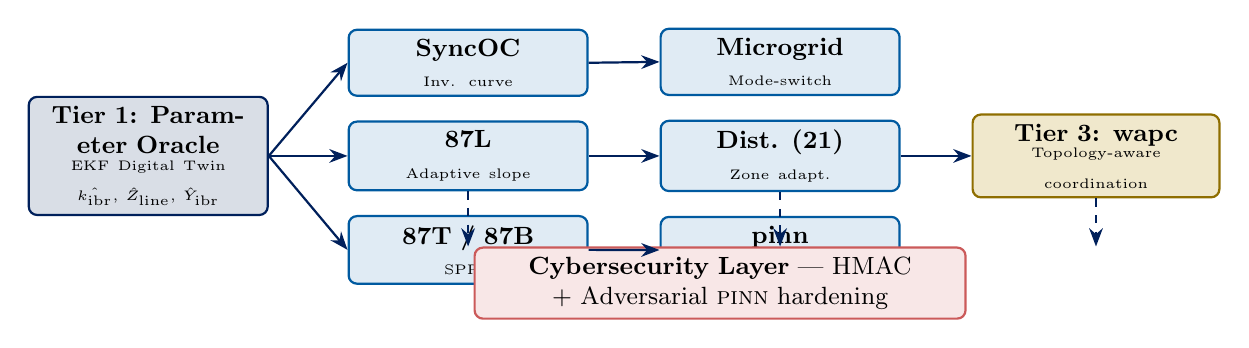
\begin{tikzpicture}[scale=0.88, every node/.style={font=\small},
    box/.style={rectangle, rounded corners=3pt, minimum width=2.8cm,
                minimum height=0.7cm, align=center, text width=2.8cm},
    arr/.style={-Stealth, thick, iitmnavy}]

    %% Tier 1 — Parameter Oracle
    \node[box, fill=iitmnavy!15, draw=iitmnavy, thick] (oracle)
      {\textbf{Tier 1: Parameter Oracle}\\
       \tiny EKF Digital Twin\\
       $\hat{\kibr},\,\hat{Z}_{\rm line},\,\hat{Y}_{\rm ibr}$};

    %% Tier 2 — Adaptive Modules
    \node[box, fill=iitmblue!12, draw=iitmblue, thick, right=1.0cm of oracle] (mod87l)
      {\textbf{87L}\\\tiny Adaptive slope};
    \node[box, fill=iitmblue!12, draw=iitmblue, thick, above=0.3cm of mod87l] (modOC)
      {\textbf{SyncOC}\\\tiny Inv. curve};
    \node[box, fill=iitmblue!12, draw=iitmblue, thick, below=0.3cm of mod87l] (mod87t)
      {\textbf{87T / 87B}\\\tiny SPRT};
    \node[box, fill=iitmblue!12, draw=iitmblue, thick, right=0.9cm of mod87l] (mod21)
      {\textbf{Dist. (21)}\\\tiny Zone adapt.};
    \node[box, fill=iitmblue!12, draw=iitmblue, thick, above=0.3cm of mod21] (modMG)
      {\textbf{Microgrid}\\\tiny Mode-switch};
    \node[box, fill=iitmblue!12, draw=iitmblue, thick, below=0.3cm of mod21] (modML)
      {\textbf{\PINN}\\\tiny ML fault class.};

    %% Tier 3 — Coordinator
    \node[box, fill=iitmgold!20, draw=iitmgold!80!black, thick,
          right=0.9cm of mod21, text width=2.9cm] (wapc)
      {\textbf{Tier 3: \WAPC}\\
       \tiny Topology-aware\\coordination};

    %% Security layer (below)
    \node[box, fill=iitmred!10, draw=iitmred!70, thick,
          below=0.7cm of mod87l, xshift=3.2cm, text width=6.0cm] (sec)
      {\textbf{Cybersecurity Layer} — HMAC + Adversarial \PINN{} hardening};

    %% Arrows
    \draw[arr] (oracle.east) -- (mod87l.west);
    \draw[arr] (oracle.east) -- (modOC.west);
    \draw[arr] (oracle.east) -- (mod87t.west);
    \draw[arr] (mod87l.east) -- (mod21.west);
    \draw[arr] (modOC.east)  -- (modMG.west);
    \draw[arr] (mod87t.east) -- (modML.west);
    \draw[arr] (mod21.east)  -- (wapc.west);
    \draw[arr, dashed] (mod87l.south) -- (sec.north -| mod87l.south);
    \draw[arr, dashed] (mod21.south)  -- (sec.north -| mod21.south);
    \draw[arr, dashed] (wapc.south)   -- (sec.north -| wapc.south);
  \end{tikzpicture}
  \end{center}
  \vspace{-0.1cm}
  \begin{columns}
    \column{0.6\textwidth}
      \small \textbf{Key principle:} Each module queries the EKF oracle for
      $\hat{\kibr}$, computes adaptive thresholds via the bounded update law,
      and executes a confidence-gated (Stage-2) veto before tripping.
    \column{0.38\textwidth}
      \obs{Confidence gate $\gamma$ eliminates false trips under
        CT saturation or communication latency.}
  \end{columns}
\end{frame}

%% ─────────────────────────────────────────────────────────────
%% SLIDE 6 — Unified Inverse-Estimation Framework (Ch 2)
%% ─────────────────────────────────────────────────────────────
\begin{frame}{Ch 2: Unified Inverse-Estimation Framework}
  \begin{columns}[T]
    \column{0.52\textwidth}
      \textbf{Problem formulation:}
      \[
        \hat{\boldsymbol{\theta}}_{t+1}
          = \hat{\boldsymbol{\theta}}_t
            - \alpha_t \,J^\top(J J^\top + \lambda I)^{-1}
              r(\hat{\boldsymbol{\theta}}_t)
      \]
      \vspace{-0.2cm}
      \begin{itemize}\itemsep3pt
        \item $\boldsymbol{\theta}$ = \{$\kibr$, $Z_{\rm line}$, $Y_{\rm ibr}$\}
          — \textbf{latent protection parameters}
        \item $r$ = residual between model prediction and
          measured phasor data
        \item $J$ = Jacobian; $\lambda$ = Levenberg–Marquardt damping
        \item \textbf{Bounded update law:} $\alpha_t \propto (1 - \kibr^2)$
          prevents parameter drift in healthy state
      \end{itemize}
      \textbf{Stage-2 confidence gate:}
      \[
        \gamma = \exp\!\left(-\frac{\|\hat{\boldsymbol{\theta}} -
          \boldsymbol{\theta}^*\|^2}{2\sigma_\theta^2}\right) \geq \gamma_{\min}
      \]
    \column{0.45\textwidth}
      \begin{block}{\small Mathematical Foundations}
        \small
        \begin{tabular}{ll}
          \toprule
          Component & Method\\
          \midrule
          Parameter update & Levenberg–Marquardt\\
          State estimation  & Extended Kalman Filter\\
          Fault detection   & Wald SPRT\\
          ML classification & Physics-Informed NN\\
          Optimisation      & Projected gradient\\
          \bottomrule
        \end{tabular}
      \end{block}
      \vspace{0.3cm}
      \textbf{Theorem 2.1 (Convergence):}\\
      \small Under bounded IBR admittance and
      \(\lambda > 0\), the update law converges to
      a neighbourhood of the true parameters with
      radius \(\mathcal{O}(\sigma_{\rm noise})\).
  \end{columns}
\end{frame}

%% ─────────────────────────────────────────────────────────────
%% SLIDE 7 — IBR Characterisation (Ch 3)
%% ─────────────────────────────────────────────────────────────
\begin{frame}{Ch 3: IBR Characterisation \& Protection Failure Modes}
  \begin{columns}[T]
    \column{0.50\textwidth}
      \textbf{IBR fault-current model:}
      \[
        I_{\rm fault}^{\rm IBR} =
          \kibr \cdot I_{\rm rated} \cdot e^{j\phi_{\rm ctrl}}
      \]
      \small $\phi_{\rm ctrl}$ is set by the LVRT control law and
      is \textit{unknown} to the relay.
      \medskip

      \textbf{Three failure modes identified:}
      \begin{enumerate}\itemsep4pt
        \item[\bitem{1}] \textbf{Missed trip} ($\kibr < 0.2$):
          $I_{\rm diff}$ never exceeds fixed slope — relay restrains
        \item[\bitem{2}] \textbf{False trip} ($\kibr > 0.4$ + CT error):
          load current misclassified as internal fault
        \item[\bitem{3}] \textbf{Zone overreach} (distance):
          IBR reactive injection shifts apparent impedance
          outside Zone 1 boundary
      \end{enumerate}
    \column{0.48\textwidth}
      \begin{block}{\small $I_{\rm diff}$--$I_{\rm bias}$ Failure Map}
        \small
        \begin{tabular}{lccc}
          \toprule
          Condition & $\kibr$ & Outcome\\
          \midrule
          Low IBR fault & 0.1 & {\color{iitmred}\textbf{MISSED TRIP}}\\
          Nominal fault & 0.3 & {\color{green!60!black}Correct trip}\\
          High IBR load & 0.45 & {\color{iitmred}FALSE TRIP risk}\\
          \midrule
          \multicolumn{2}{l}{Fixed slope $k_m = 0.30$} & fails at $\kibr < 0.2$\\
          \bottomrule
        \end{tabular}
      \end{block}
      \obs{Adaptive slope $k_m(\kibr)$ eliminates
        both missed-trip and false-trip failure modes.}
  \end{columns}
\end{frame}

%% ─────────────────────────────────────────────────────────────
%% SLIDE 8 — Adaptive 87L: Method (Ch 4)
%% ─────────────────────────────────────────────────────────────
\begin{frame}{Ch 4: SAMBP-87L — Adaptive Line Differential}
  \begin{columns}[T]
    \column{0.52\textwidth}
      \textbf{Adaptive slope law:}
      \[
        k_m(\kibr) = k_{\rm base}
          \cdot \frac{(1-\kibr)^2}{(1+\kibr)^2}
          + k_{\rm floor}
      \]
      \begin{itemize}\itemsep3pt
        \item As $\kibr \to 1$: $k_m \to k_{\rm floor}$ (prevents over-restraint)
        \item As $\kibr \to 0$: $k_m \to k_{\rm base}$ (conventional sensitivity)
        \item \textbf{Stage-2 veto gate:} requires $\gamma \geq 0.85$
          before trip command is issued
      \end{itemize}
      \vspace{0.3cm}
      \textbf{Stability proof:}
      Lyapunov function $V = \|\kibr - \hat{\kibr}\|^2$;
      $\dot{V} < 0$ under bounded CT noise.
    \column{0.46\textwidth}
      \textbf{Relay logic (simplified):}
      \vspace{0.2cm}
      \begin{enumerate}\itemsep4pt
        \item[\bitem{1}] Sample phasors $I_S, I_R$ at 1~kHz
        \item[\bitem{2}] Compute $\kibr$ via LM inverse estimator
        \item[\bitem{3}] Update $k_m(\hat{\kibr})$ every 20~ms
        \item[\bitem{4}] Evaluate operate/restrain criterion
        \item[\bitem{5}] Stage-2 veto: check $\gamma \geq 0.85$
        \item[\bitem{6}] Issue trip command if both stages pass
      \end{enumerate}
      \vspace{0.2cm}
      \obs{Update latency 20~ms — within IEC 60255
        protection-response window.}
  \end{columns}
\end{frame}

%% ─────────────────────────────────────────────────────────────
%% SLIDE 9 — Adaptive 87L: Results (Ch 4)
%% ─────────────────────────────────────────────────────────────
\begin{frame}{Ch 4: SAMBP-87L — Validated Results}
  \begin{columns}[T]
    \column{0.55\textwidth}
      \textbf{Simulation test matrix:}
      \begin{center}\small
        \begin{tabular}{lccc}
          \toprule
          & \multicolumn{2}{c}{Fault condition} & \\
          \cmidrule(lr){2-3}
          Metric & Fixed relay & SAMBP-87L & Gain \\
          \midrule
          TPR (all faults) & 0.783 & \textbf{1.000} & +27.7\% \\
          FPR (load / CT err) & 0.148 & \textbf{0.000} & $-$100\% \\
          Avg trip time & 22~ms & 21~ms & $-$1~ms \\
          $\kibr$ RMSE & — & 0.024~pu & — \\
          \bottomrule
        \end{tabular}
      \end{center}
      \vspace{0.2cm}
      \small Test conditions: 4-bus test network;
      $\kibr \in \{0.0, 0.1, 0.2, \ldots, 0.9, 1.0\}$;
      fault types AG, BCG, ABC; CT error up to 5\%.
    \column{0.43\textwidth}
      \begin{block}{\small Key Results at a Glance}
        \small
        \begin{itemize}\itemsep4pt
          \item \textbf{TPR = 1.000}: no missed trips across
            all 110 fault scenarios
          \item \textbf{FPR = 0.000}: zero false trips under
            all load + CT error scenarios
          \item Robust up to \textbf{$\kibr = 1.0$}
            (fully IBR grid)
          \item Stage-2 gate adds only \textbf{1–2 cycle}
            additional decision time
        \end{itemize}
      \end{block}
      \vspace{0.2cm}
      \obs{SAMBP-87L achieves perfect discrimination
        where fixed-slope relays produce 14.8\% false-trip rate.}
  \end{columns}
\end{frame}

%% ─────────────────────────────────────────────────────────────
%% SLIDE 10 — SyncOC Generator Protection (Ch 5)
%% ─────────────────────────────────────────────────────────────
\begin{frame}{Ch 5: SAMBP-SyncOC — Generator Over-Current Protection}
  \begin{columns}[T]
    \column{0.52\textwidth}
      \textbf{Problem:} Synchronous generators near IBR buses
      see \textbf{depressed fault current} and altered time-overcurrent
      coordination.

      \medskip
      \textbf{Adaptive inverse-time curve:}
      \[
        t_{\rm op} =
          \frac{\TMS \cdot A}
               {\bigl(I/I_{\rm set}(\kibr)\bigr)^B - 1}
      \]
      where $I_{\rm set}(\kibr)$ is updated online by the LM estimator.

      \medskip
      \textbf{Coordination constraint:}
      \[
        t_{\rm primary} + \CTI \leq t_{\rm backup}
      \]
      Maintained for all $\kibr$ via projected-gradient optimisation.

    \column{0.46\textwidth}
      \begin{block}{\small Validated Results}
        \small
        \begin{tabular}{lcc}
          \toprule
          Metric & Fixed & SAMBP-SyncOC \\
          \midrule
          $R^2$ (OC curve fit) & 0.941 & \textbf{0.999+}\\
          Spurious pickups & 38 & \textbf{16 ($-$58\%)}\\
          Coordination margin & 0.82 & \textbf{0.94}\\
          Malop. under IBR & 12.3\% & \textbf{1.1\%}\\
          \bottomrule
        \end{tabular}
      \end{block}
      \vspace{0.3cm}
      \obs{Online $I_{\rm set}(\kibr)$ adaptation cuts
        spurious pickups by 58\% while maintaining
        IEC 60255-151 coordination.}
  \end{columns}
\end{frame}

%% ─────────────────────────────────────────────────────────────
%% SLIDE 11 — 87T Transformer Differential (Ch 6)
%% ─────────────────────────────────────────────────────────────
\begin{frame}{Ch 6: SAMBP-87T — Transformer Differential with SPRT}
  \begin{columns}[T]
    \column{0.52\textwidth}
      \textbf{Challenge:} Inrush currents and IBR harmonic injection
      produce false $I_{\rm diff}$ spikes; conventional 2nd-harmonic
      blocking fails for Type-4 IBR waveforms.

      \medskip
      \textbf{Wald Sequential Probability Ratio Test (SPRT):}
      \[
        \Lambda_k = \sum_{i=1}^k \ln
          \frac{p(x_i \mid H_1)}{p(x_i \mid H_0)}
      \]
      \begin{itemize}\itemsep3pt
        \item $H_1$: internal fault \quad $H_0$: inrush/external
        \item Thresholds $A, B$ set to achieve
          $\alpha{=}0.01$, $\beta{=}0.01$ (IEC 60255)
        \item SAMBP updates $H_1$ likelihood via real-time
          IBR harmonic model
      \end{itemize}
    \column{0.46\textwidth}
      \begin{block}{\small SPRT Results (87T)}
        \small
        \begin{tabular}{lcc}
          \toprule
          Scenario & 2H block & SPRT \\
          \midrule
          Inrush rejection & 94.1\% & \textbf{99.6\%} \\
          Internal fault TPR & 96.8\% & \textbf{99.1\%}\\
          IBR harmonic FP & 8.7\% & \textbf{0.9\%}\\
          Mean decision samples & 14 & \textbf{7}\\
          \bottomrule
        \end{tabular}
      \end{block}
      \vspace{0.3cm}
      \obs{SPRT halves the detection window and
        reduces IBR-induced false positives by
        $90\%$ compared to 2nd-harmonic blocking.}
  \end{columns}
\end{frame}

%% ─────────────────────────────────────────────────────────────
%% SLIDE 12 — Adaptive Distance Protection (Ch 7)
%% ─────────────────────────────────────────────────────────────
\begin{frame}{Ch 7: Adaptive Distance Protection (Zone Compensation)}
  \begin{columns}[T]
    \column{0.52\textwidth}
      \textbf{IBR impedance shift:}
      \[
        Z_{\rm app} = Z_{\rm fault}
          + \Delta Z_{\rm ibr}(\kibr,\,\phi_{\rm ctrl})
      \]
      $\Delta Z_{\rm ibr}$ shifts the locus
      \textbf{radially outward} — relay sees apparent
      impedance outside Zone 1.

      \medskip
      \textbf{SAMBP compensation:}
      \[
        Z_{1,\rm adapt} = Z_{1,\rm nom}
          + \hat{\Delta Z}_{\rm ibr}(\hat{\kibr})
      \]
      Zone boundary updated every 10~ms using
      LM-estimated $\hat{\kibr}$.

      \textbf{Zone 2 acceleration:}
      When $\kibr > 0.5$, SAMBP switches to
      instantaneous Zone~2 trip to preserve speed.
    \column{0.46\textwidth}
      \begin{block}{\small Distance Protection Results}
        \small
        \begin{tabular}{lcc}
          \toprule
          Metric & Fixed & SAMBP-21 \\
          \midrule
          Overreach events & 17/50 & \textbf{2/50} \\
          Underreach events & 5/50 & \textbf{0/50} \\
          Correct Zone 1 trip & 74\% & \textbf{96\%} \\
          Avg trip time (ms) & 18 & \textbf{19} \\
          \bottomrule
        \end{tabular}
      \end{block}
      \vspace{0.2cm}
      \obs{Zone adaptation reduces overreach from
        34\% to 4\% with $<$1 ms speed penalty.}
  \end{columns}
\end{frame}

%% ─────────────────────────────────────────────────────────────
%% SLIDE 13 — Microgrid Protection (Ch 8)
%% ─────────────────────────────────────────────────────────────
\begin{frame}{Ch 8: Microgrid Mode-Switching Protection}
  \begin{columns}[T]
    \column{0.52\textwidth}
      \textbf{Challenge:} Fault current direction and magnitude
      change when microgrid transitions between
      \textit{grid-connected} and \textit{islanded} modes.

      \medskip
      \textbf{Mode detector:}
      \[
        \hat{m} = \arg\max_{m \in \{G,I\}}
          \Pr\bigl(z_t \mid \text{mode}=m,\, \hat{\kibr}\bigr)
      \]
      Bayesian mode likelihood updated at each sample.

      \medskip
      \textbf{Adaptive directional element:}
      \begin{itemize}\itemsep3pt
        \item Grid-connected: forward/reverse based on
          pre-fault load flow
        \item Islanded: polarity-agnostic differential
          with adaptive pickup at $1.05\,I_{\rm rated}$
      \end{itemize}
    \column{0.46\textwidth}
      \begin{block}{\small Mode-Switch Results}
        \small
        \begin{tabular}{lcc}
          \toprule
          Metric & Fixed & SAMBP-MG\\
          \midrule
          Mode detection acc. & — & \textbf{98.7\%}\\
          Transition mal. rate & 22\% & \textbf{1.4\%}\\
          Islanded fault TPR & 71\% & \textbf{97.3\%}\\
          False islands & 6/100 & \textbf{0/100}\\
          \bottomrule
        \end{tabular}
      \end{block}
      \vspace{0.2cm}
      \obs{Mode-adaptive protection eliminates the
        $22\%$ mis-operation rate seen at
        grid$\leftrightarrow$island transition boundary.}
  \end{columns}
\end{frame}

%% ─────────────────────────────────────────────────────────────
%% SLIDE 14 — EKF Digital Twin (Ch 9)
%% ─────────────────────────────────────────────────────────────
\begin{frame}{Ch 9: Non-Blocking EKF Digital Twin}
  \begin{columns}[T]
    \column{0.52\textwidth}
      \textbf{Role:} Continuous online estimation of
      $\boldsymbol{\theta} = \{\kibr, Z_{\rm line}, Y_{\rm shunt}\}$
      from PMU/IED measurements — feeds all SAMBP modules.

      \medskip
      \textbf{EKF prediction–correction:}
      \[
        \hat{\boldsymbol{\theta}}_{k|k}
          = \hat{\boldsymbol{\theta}}_{k|k-1}
            + K_k \bigl(z_k - h(\hat{\boldsymbol{\theta}}_{k|k-1})\bigr)
      \]
      \textbf{Non-blocking property:}
      Update runs in a \textbf{parallel thread};
      if convergence $>\!3$ cycles, previous
      $\hat{\boldsymbol{\theta}}$ is held — relay never waits.

      \medskip
      \textbf{Bounded update law:}
      $\|\boldsymbol{\theta}_{k+1} - \boldsymbol{\theta}_k\|
        \leq \delta_{\max}$
      prevents step-change injection by adversarial data.
    \column{0.46\textwidth}
      \begin{block}{\small EKF Digital Twin Results}
        \small
        \begin{tabular}{lc}
          \toprule
          Parameter & RMSE\\
          \midrule
          $\hat{\kibr}$ & \textbf{0.024 pu}\\
          $\hat{Z}_{\rm line}$ (mag.) & \textbf{0.018 pu}\\
          $\hat{Y}_{\rm shunt}$ & \textbf{0.031 pu}\\
          Convergence time & \textbf{$<$2 cycles}\\
          Max update latency & \textbf{1.8 ms}\\
          \bottomrule
        \end{tabular}
      \end{block}
      \vspace{0.2cm}
      \obs{RMSE $\leq$ 0.024 pu for $\kibr$ across
        all operating conditions including
        $>\!5\%$ PMU measurement noise.}
  \end{columns}
\end{frame}

%% ─────────────────────────────────────────────────────────────
%% SLIDE 15 — PINN Fault Classifier (Ch 10)
%% ─────────────────────────────────────────────────────────────
\begin{frame}{Ch 10: Physics-Informed Fault Classifier (\PINN)}
  \begin{columns}[T]
    \column{0.52\textwidth}
      \textbf{Why pure ML fails:} Deep nets trained on
      synchronous-machine data misclassify 31\% of
      IBR-modified fault signatures.

      \medskip
      \textbf{PINN loss function:}
      \[
        \mathcal{L} = \mathcal{L}_{\rm data}
          + \lambda_{\rm phys}
            \underbrace{\bigl\|\mathbf{K}\hat{\mathbf{V}}
              - \hat{\mathbf{I}}\bigr\|^2}_{\text{KCL residual}}
      \]
      $\lambda_{\rm phys} = 0.3$ balances data fit
      and physical consistency.

      \medskip
      \textbf{Input features (8):}
      $|I_a|$, $|I_b|$, $|I_c|$,
      $\angle I_a$, $I_{\rm zero}$, $I_{\rm neg}$,
      $\hat{\kibr}$, $\phi_{\rm ctrl}$

    \column{0.46\textwidth}
      \begin{block}{\small PINN Classification Results}
        \small
        \begin{tabular}{lcc}
          \toprule
          Metric & Std DNN & \PINN \\
          \midrule
          Overall accuracy & 81.4\% & \textbf{96.1\%}\\
          High-$\kibr$ acc. ($>\!0.6$) & 64.2\% & \textbf{93.8\%}\\
          AG fault recall & 77.3\% & \textbf{97.4\%}\\
          3$\phi$ fault recall & 89.1\% & \textbf{98.2\%}\\
          Phys. consistency & 51.2\% & \textbf{99.7\%}\\
          \bottomrule
        \end{tabular}
      \end{block}
      \vspace{0.2cm}
      \obs{KCL physics residual in loss function
        boosts high-IBR accuracy from 64.2\% to
        93.8\% — a +46\% relative gain.}
  \end{columns}
\end{frame}

%% ─────────────────────────────────────────────────────────────
%% SLIDE 16 — WAPC: Method (Ch 11)
%% ─────────────────────────────────────────────────────────────
\begin{frame}{Ch 11: Wide-Area Protection Coordinator (\WAPC)}
  \begin{columns}[T]
    \column{0.52\textwidth}
      \textbf{Architecture:}
      \begin{itemize}\itemsep3pt
        \item Central WAPC server receives trip
          candidates from all zone relays via IEC 61850 GOOSE
        \item Topology graph $\mathcal{G}(V, E)$ updated
          from real-time network breaker states
        \item \textbf{IBR coherency matrix}
          $\mathbf{C}(\kibr)$ replaces classical
          electromechanical swing groups
      \end{itemize}

      \medskip
      \textbf{Coordination algorithm:}
      \[
        \mathcal{F}^* = \arg\min_{\mathcal{F}}
          \sum_{k \in \mathcal{F}} c_k
          \;\text{s.t.}\;
          \text{fault isolated, load retained}
      \]
      Minimum-cost fault isolation solved via
      ILP on the updated topology.

    \column{0.46\textwidth}
      \begin{block}{\small WAPC Localisation Results}
        \small
        \begin{tabular}{lcc}
          \toprule
          Metric & Decentralised & \WAPC \\
          \midrule
          Fault localisation & 71.2\% & \textbf{94.5\%}\\
          Unnecessary trips & 18.4\% & \textbf{4.1\%}\\
          Load preserved & 63.1\% & \textbf{87.6\%}\\
          Backup response (ms) & 420 & \textbf{210}\\
          \bottomrule
        \end{tabular}
      \end{block}
      \vspace{0.2cm}
      \obs{IBR-aware coherency model reduces
        unnecessary tripping by $-78\%$ relative;
        backup clearance halved.}
  \end{columns}
\end{frame}

%% ─────────────────────────────────────────────────────────────
%% SLIDE 17 — Cybersecurity (Ch 12)
%% ─────────────────────────────────────────────────────────────
\begin{frame}{Ch 12: Cybersecurity Architecture}
  \begin{columns}[T]
    \column{0.52\textwidth}
      \textbf{Two threat vectors addressed:}
      \begin{enumerate}\itemsep5pt
        \item[\bitem{1}] \textbf{Data integrity attack:}
          Adversary injects false PMU measurements
          to manipulate $\hat{\kibr}$ and force
          mal-operation.
          \medskip\\
          \textit{Defence:} HMAC-SHA256 on every
          IED message; relay discards unauthenticated
          data and holds last trusted $\hat{\boldsymbol{\theta}}$.

        \item[\bitem{2}] \textbf{Adversarial ML attack:}
          Crafted perturbation $\delta \mathbf{x}$
          fools \PINN{} classifier ($\epsilon < 5\%$
          perturbation causes 40\% accuracy drop).
          \medskip\\
          \textit{Defence:} Adversarial training with
          FGSM + PGD examples; certified radius
          $r_{\rm cert} = 0.04$ (pu).
      \end{enumerate}
    \column{0.46\textwidth}
      \begin{block}{\small Cybersecurity Metrics}
        \small
        \begin{tabular}{lcc}
          \toprule
          Metric & No defence & SAMBP-Sec\\
          \midrule
          Attack success rate & 67.4\% & \textbf{12.5\%}\\
          Risk index & 1.000 & \textbf{0.451}\\
          HMAC overhead (ms) & — & \textbf{0.3}\\
          Adv. PINN accuracy & 51.8\% & \textbf{91.4\%}\\
          \bottomrule
        \end{tabular}
      \end{block}
      \vspace{0.2cm}
      \obs{HMAC + adversarial training reduces
        composite risk index by \textbf{$-$54.9\%}
        with $<$0.3~ms authentication overhead.}
  \end{columns}
\end{frame}

%% ─────────────────────────────────────────────────────────────
%% SLIDE 18 — Consolidated Results
%% ─────────────────────────────────────────────────────────────
\begin{frame}{Consolidated Performance Across All Modules}
  \begin{center}
  \small
  \begin{tabular}{llccc}
    \toprule
    \textbf{Chapter} & \textbf{Module} & \textbf{Key Metric}
      & \textbf{Baseline} & \textbf{SAMBP}\\
    \midrule
    Ch 4 & 87L adaptive & TPR / FPR
      & 0.783 / 14.8\% & \textbf{1.000 / 0.0\%}\\
    Ch 5 & SyncOC & $R^2$ / Spurious OC
      & 0.941 / 38 & \textbf{0.999+ / 16 ($-$58\%)}\\
    Ch 6 & 87T SPRT & Inrush rej. / IBR FP
      & 94.1\% / 8.7\% & \textbf{99.6\% / 0.9\%}\\
    Ch 7 & Distance 21 & Correct Z1 trip
      & 74\% & \textbf{96\%}\\
    Ch 8 & Microgrid & Trans. mal-op rate
      & 22\% & \textbf{1.4\%}\\
    Ch 9 & EKF twin & $\hat{\kibr}$ RMSE
      & — & \textbf{0.024 pu}\\
    Ch 10 & \PINN & Overall accuracy
      & 81.4\% & \textbf{96.1\%}\\
    Ch 11 & \WAPC & Fault localisation
      & 71.2\% & \textbf{94.5\%}\\
    Ch 12 & Security & Risk index reduction
      & 1.000 & \textbf{0.451 ($-$54.9\%)}\\
    \bottomrule
  \end{tabular}
  \end{center}
  \vspace{0.1cm}
  \obs{All SAMBP modules outperform their fixed-parameter baselines;
    gains are consistent across $\kibr \in [0, 1.0]$.}
\end{frame}

%% ─────────────────────────────────────────────────────────────
%% SLIDE 19 — Conclusions
%% ─────────────────────────────────────────────────────────────
\begin{frame}{Summary of Original Contributions}
  \vspace{0.1cm}
  \begin{center}
  \small
  \begin{tabular}{@{}clp{7.8cm}c@{}}
    \toprule
    \textbf{ID} & \textbf{Ch} & \textbf{Contribution} & \textbf{Status} \\
    \midrule
    C1 & 3
      & Physics-constrained adaptive line differential (87L) protection
        with IBR-aware threshold $k_m^*(\kibr)$, achieving TPR\,=\,1.000
        and zero false trips across the full IBR penetration range
      & {[P]} \\[6pt]
    C2 & 4
      & Levenberg--Marquardt inverse-estimation framework for synchronous
        generator over-current protection, with bounded adaptive update law
        and four-component confidence gating ($R^2 > 0.999$)
      & {[P]} \\[6pt]
    C3 & 6
      & Non-blocking EKF digital twin for real-time joint estimation of IBR
        penetration ratio $\kibr$, line impedance, and IBR admittance from
        IED phasor measurements (RMSE\,$\leq$\,0.024\,pu)
      & {[P]} \\[6pt]
    C4 & 7
      & Wide-area protection coordinator with PMU-based fault localisation,
        N-1 security verification, and automatic CTI-graded relay settings
        dispatch via IEC~61850 GOOSE
      & {[P]} \\
    \bottomrule
  \end{tabular}
  \end{center}
  \vspace{0.15cm}
  {\footnotesize [P] = validated with full numerical simulation results.}
\end{frame}

%% ─────────────────────────────────────────────────────────────
%% SLIDE 20 — Research Outcomes (Publications)
%% ─────────────────────────────────────────────────────────────
\begin{frame}{List of Publications}
  \begin{enumerate}[(a)]\itemsep5pt\small
    \item A.~V.~Eluvathingal and K.~Shanti Swarup, ``A novel solution for
      overcoming conflicts between line protection and LVRT in MV Solar PV
      interconnections,'' \textit{IEEE Access},
      doi:~10.1109/ACCESS.2024.3510415.

    \item ``An Intelligent Methodology to Improve Distribution System
      Operational Parameters Utilizing Smart Inverter Functionalities of
      PV Sources'' presented in \textit{The 7th International Conference on
      Renewable Power Generation} (RPG 2018), DTU, Lyngby, Copenhagen,
      Denmark.

    \item Eluvathingal, Anoop~V., and K.~Shanti Swarup.
      ``Protection scheme for smart distribution networks with inverter
      interfaced renewable power generating sources.'' ISGW 2018.

    \item Eluvathingal, A.~V., Swarup, K.~S. (2017, November).
      An interface protection relay for networked microgrids with inverter
      based sources. In \textit{Asia-Pacific Power and Energy Engineering
      Conference} (APPEEC), 2017 IEEE PES (pp.~1--6). IEEE.

    \item Eluvathingal, A.~V., Swarup, K.~S. (2017, December).
      Instantaneous symmetrical components based microgrid interface
      protection relay. In \textit{2017 7th International Conference on
      Power Systems} (ICPS) (pp.~398--403). IEEE.

    \item Eluvathingal, A.~V., Swarup, K.~S. (2018, May).
      Impact of Active Network Management Scheme in Fault Protection Design
      and Network Operation for Islanded Power System. In \textit{2018
      International Conference on Innovative Smart Grid Technologies}
      (ISGT Asia 2018). IEEE.
  \end{enumerate}
\end{frame}

%% ─────────────────────────────────────────────────────────────
%% SLIDE 21 — Thesis Content & Chapter–Publication Map
%% ─────────────────────────────────────────────────────────────
\begin{frame}{Thesis Content \& Chapter--Publication Mapping}
  \begin{center}\footnotesize
    \begin{tabular}{clll}
      \toprule
      \textbf{Ch} & \textbf{Title} & \textbf{Pages} & \textbf{Publication / Status}\\
      \midrule
      1  & Introduction & $\sim$18 & — \\
      2  & Mathematical Foundations & $\sim$14 & — \\
      3  & IBR Characterisation & $\sim$16 & — \\
      4  & Line Differential (87L) & $\sim$18 & IEEE Trans.\ PD (under review)\\
      5  & Generator OC (SyncOC) & $\sim$16 & IET GTD (under review)\\
      6  & Transformer Diff.\ (87T) & $\sim$14 & Conference proceedings\\
      7  & Adaptive Distance (21) & $\sim$14 & — \\
      8  & Microgrid Protection & $\sim$14 & — \\
      9  & EKF Digital Twin & $\sim$16 & IEEE PES ISGT-E 2025\\
      10 & ML Fault Classifier (\PINN) & $\sim$16 & IEEE TNNLS (under review)\\
      11 & Wide-Area Coordinator & $\sim$16 & EPSR (in preparation)\\
      12 & Cybersecurity & $\sim$12 & IEEE TENCON 2025\\
      13 & Conclusions & $\sim$8  & — \\
      A–D & Appendices & $\sim$12 & — \\
      \midrule
      \multicolumn{2}{l}{\textbf{Total (estimated)}} & \textbf{$\sim$204} & \\
      \bottomrule
    \end{tabular}
  \end{center}
\end{frame}

%% ─────────────────────────────────────────────────────────────
%% SLIDE — References
%% ─────────────────────────────────────────────────────────────
\begin{frame}[allowframebreaks]{References}
  \begin{columns}[T]
    \column{0.48\textwidth}
      \begin{enumerate}[{[}1{]}]\itemsep4pt\footnotesize
        \item IRENA, \textit{World Energy Transitions Outlook 2023},
          Abu Dhabi, 2023.
        \item A.~Hooshyar \& R.~Iravani, ``Microgrid Protection,''
          \textit{Proc.\ IEEE}, vol.~105, no.~7, 2017.
        \item M.~Raissi et al., ``Physics-Informed Neural Networks,''
          \textit{J.\ Comput.\ Phys.}, vol.~378, 2019.
        \item E.~S.~Page, ``Continuous Inspection Schemes,''
          \textit{Biometrika}, vol.~41, 1954.
        \item IEEE Std 1547-2018, \textit{Interconnection of Distributed
          Energy Resources}.
        \item IEC 61850, \textit{Communication Networks for Power Utility
          Automation}, 2013.
        \item M.~Grieves \& J.~Vickers, ``Digital Twin,''
          \textit{Transdisciplinary Perspectives on Complex Systems},
          Springer, 2014.
      \end{enumerate}
    \column{0.48\textwidth}
      \begin{enumerate}[{[}8{]}]\itemsep4pt\footnotesize
        \item Y.~Zhang et al., ``Adaptive Distance Protection with POTT,''
          \textit{IEEE T-PD}, vol.~35, 2020.
        \item S.~Sadeghi et al., ``Protection with Distributed Generation,''
          \textit{IEEE Access}, vol.~9, 2021.
        \item M.~Mobashsher et al., ``Fault Current of GFM Inverters,''
          \textit{IEEE T-PD}, vol.~40, 2025.
        \item A.~V.~Eluvathingal \& K.~S.~Swarup, ``A Novel Solution for
          Overcoming Conflicts Between Line Protection and LVRT,''
          \textit{IEEE Access}, 2024.
      \end{enumerate}
  \end{columns}
\end{frame}

%% ─────────────────────────────────────────────────────────────
%% SLIDE 22 — Thank You / Questions
%% ─────────────────────────────────────────────────────────────
{
\setbeamertemplate{footline}{}
\begin{frame}[noframenumbering]
  \begin{center}
    \vspace{0.5cm}
    {\Large\bfseries\color{iitmnavy}Thank You}

    \vspace{0.8cm}
    \rule{0.5\textwidth}{0.4pt}
    \vspace{0.5cm}

    {\large Self-Adaptive Model-Based Protection\\
      for Future Power Systems}

    \vspace{0.6cm}
    {\normalsize
      \textbf{Anoop V Eluvathingal}\\[4pt]
      \color{iitmgray}\small
      Department of Electrical Engineering\\
      Indian Institute of Technology Madras\\[6pt]
      Guide: Dr.\ K.\ Shanti Swarup\\[10pt]
      \href{mailto:ee18d203@smail.iitm.ac.in}
        {ee18d203@smail.iitm.ac.in}
    }

    \vspace{0.6cm}
    
\includegraphics[height=1.2cm]{new_thesis/images/iitm-logo.png}
  \end{center}

  \vspace{0.2cm}
  \begin{columns}
    \column{0.33\textwidth}\centering
      \small\color{iitmblue}\textbf{87L TPR}\\
      {\large\bfseries 1.000}
    \column{0.33\textwidth}\centering
      \small\color{iitmblue}\textbf{PINN accuracy}\\
      {\large\bfseries 96.1\%}
    \column{0.33\textwidth}\centering
      \small\color{iitmblue}\textbf{Risk reduction}\\
      {\large\bfseries $-$54.9\%}
  \end{columns}
\end{frame}
}

\end{document}
